De acuerdo con \cite{IR-book} Recuperación de Información, o IR por sus siglas en inglés hace referencia a encontrar material que satisfaga una necesidad de información. Usualmente, este material son documentos de texto y se almacena en computadores. Hasta hace algunos años esta actividad se limitaba a algunas profesiones específicas. No obstante, el \textit{boom} del internet ha ocasionado que la mayoría de estas búsquedas se hagan a través de este, sea mediante motores de búsqueda o correo electrónico.\\

Para IR se han propuesto diferentes métodos que permiten solucionar el problema desde diferentes ángulos, dentro de los cuales se encuentran búsqueda binaria, el retorna todos los documentos que cumplan cierta condición, como que contenga todos los términos buscados o al menos uno de ellos. Otra técnica es búsqueda clasificada, el cual retorna ordenadamente los documentos considerados relevantes. En el presente documento se explican algunas técnicas implementadas por los autores y una comparación de los resultados obtenidos por cada una de estas.\\

\subsection*{\textit{Dataset}}

El \textit{dataset} utilizado para el desarrollo de esta comparación consiste de un total de 331 documentos y 35 consultas (\textit{queries}) con sus respectivas etiquetas. Los documentos y las consultas están almacenados en formato \url{.naf}, por lo que se utiliza una librería de lectura de archivos \url{.xml} para ello. Por su parte, las etiquetas vienen almacenadas en archivos \url{.tsv}, los cuales son un documentos con valores separados por 't'. Para la lectura de estos se utiliza la librería \textit{pandas}.\\

Cada documento tiene un encabeza en donde se encuentra el título asociado al texto contenido, un identificador (\textit{id}) y una dirección de donde fue obtenido. Por último se encuentra el texto correspondiente. Cabe resaltar que en el texto se encuentra incluido el título del documento, razón por la cual no se incluye de manera adicional. Las consultas están organizadas de manera similar, pero sin título y con los términos clave en el lugar donde estaría el texto.

Las etiquetas de cada una de las consultas indican los documentos que resultan relevantes para esa consulta y un puntaje de 2 a 5 clasificando la relevancia del documento.

\subsection*{Preprocesamiento}

Antes de implementar las distintas estrategias de recuperación de información, se realizo un preprocesamiento igual a todo el \textit{dataset}. Con este proceso se busca representar tanto los \textit{queries} como los documentos de forma numérica de manera tal que dicha representación ayude a resolver el problema de IR. Para esto se le aplicaron distintos procesamientos estándar, los cuales se presentan de forma resumida en la figura \ref{fig:preprocess}. Todo el código correspondiente a esta sección se encuentra en el cuaderno \texttt{HW01\_Utilities.ipynb}.

\begin{figure}[H]
    \centering
    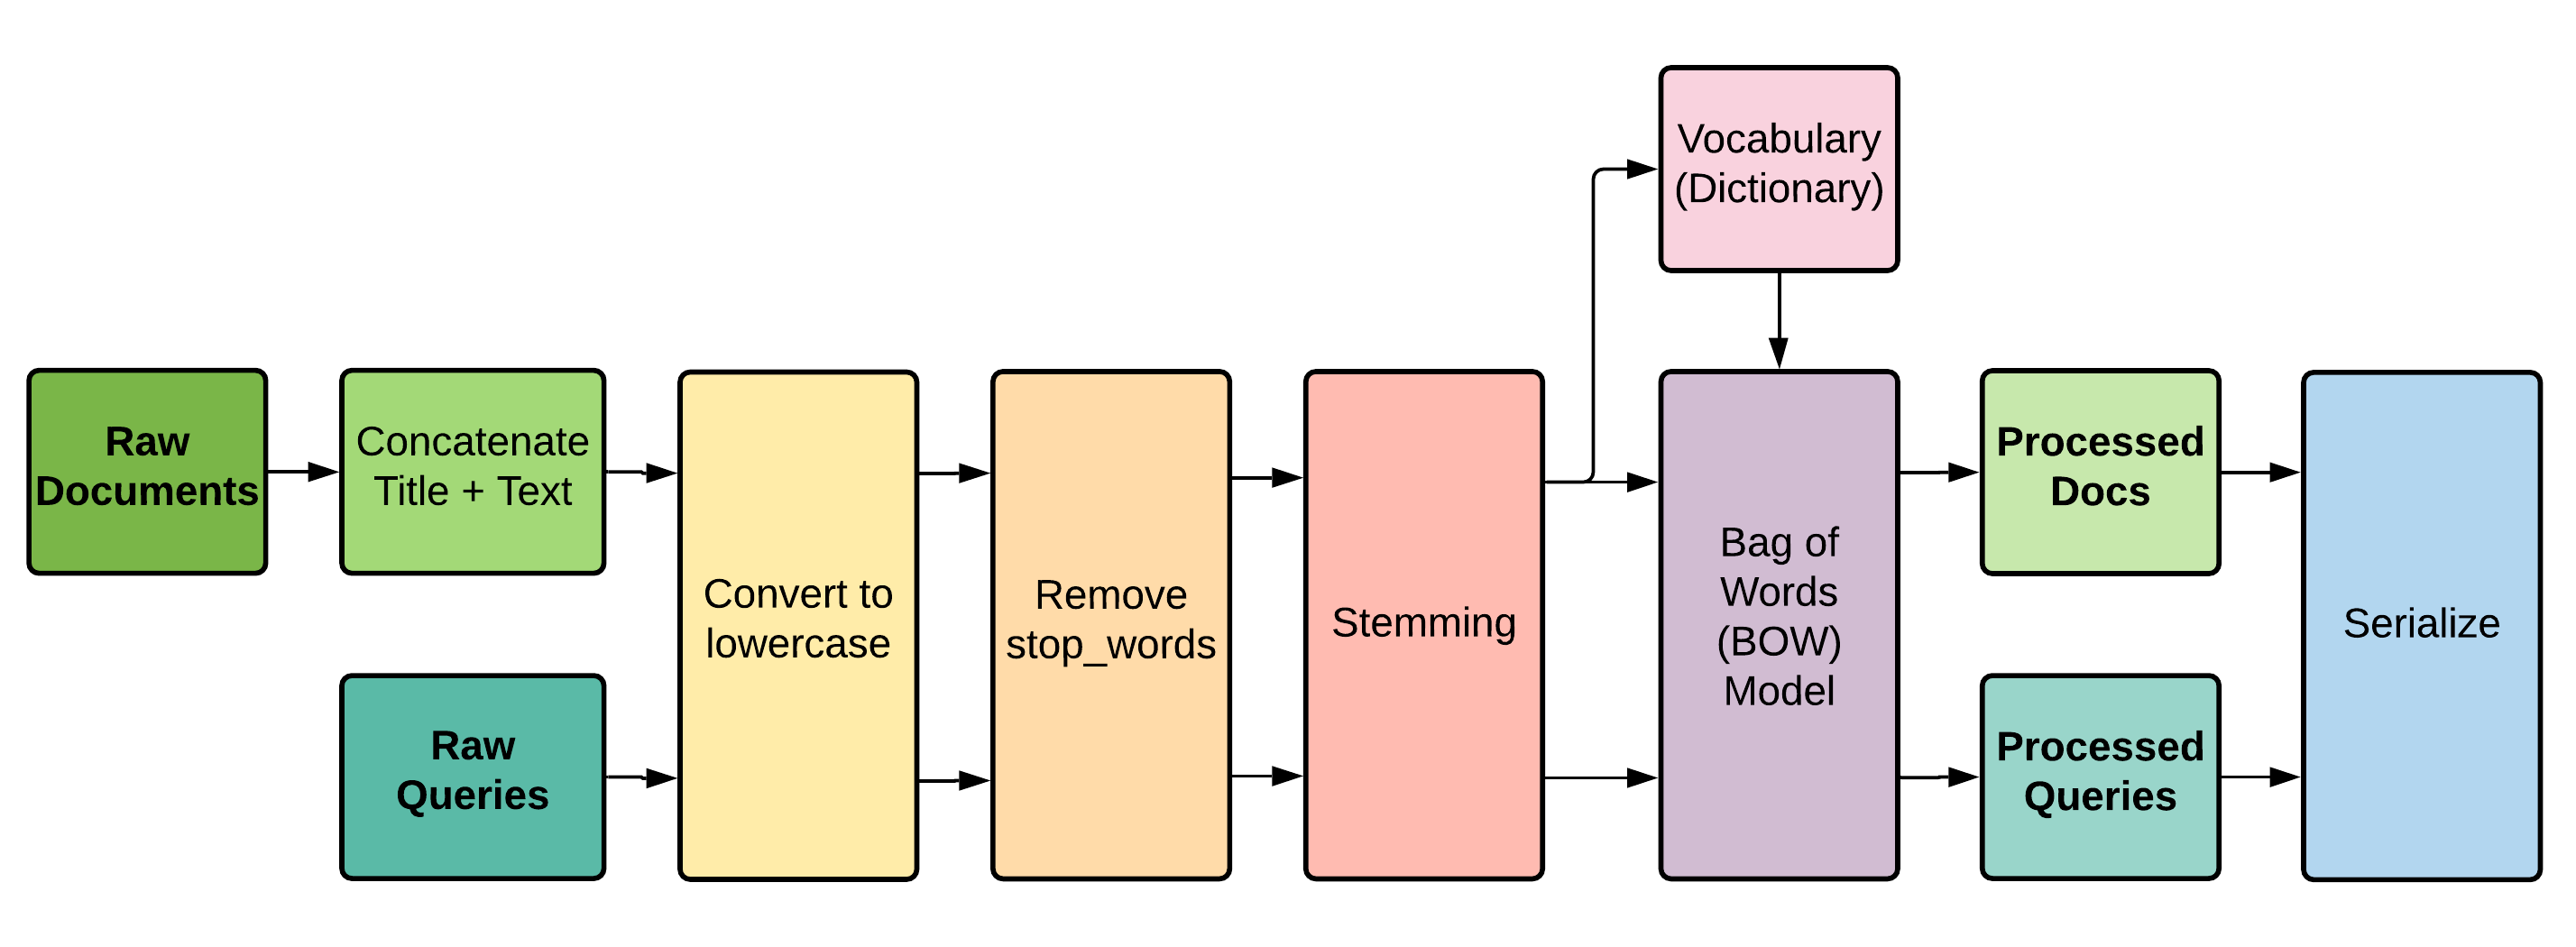
\includegraphics[width=0.95\textwidth]{doc/images/preprocesamiento.png}
    \caption{Etapas de procesamiento aplicadas al texto para resolver el problema de IR}
    \label{fig:preprocess}
\end{figure}

A grande rasgos lo que se hace es tomar el texto crudo (para los documentos se concatena el titulo con su cuerpo) y se convierten todos los caracteres a minúscula. Posteriormente, se remueven las \textit{stop words} (palabras comunes para el idioma inglés) y se reducen todas las palabras a su raíz con \textit{stemming}, todo esto con la librería \texttt{gensim.parsing} y las funciones de \texttt{remove\_stopwords} y \texttt{PorterStemer}, respectivamente. Vale la pena aclarar, que el proceso de \textit{stemming} no reduce las palabras a su raíz semántica sino con una serie de reglas establecidas para el idioma. Finalmente, con los términos (únicamente de el corpus de documentos) se construye el vocabulario (o \textit{dictionary}) y a partir de este los modelos de Bag of words (BOW), tanto para los documentos como para los \textit{queries}. Por último, estos se serializan para poder utilizarse en los distintos cuadernos donde se implementan las distintas estrategias de recuperación de información.

\subsection*{Organización del contenido}
Por facilidad, el desarrollo del presente proyecto se llevó acabo utilizando un repositorio \textit{online} de GitHub, disponible en el en \url{https://github.com/ISIS4221-JCN/HW01}.\\

El contenido del repositorio se explica a continuación:
\begin{itemize}
    \item \textbf{doc/:} Carpeta con los archivos necesarios para el informe escrito.
    \item \textbf{resources/:} Carpeta que contiene las instrucciones del proyecto y los archivos relacionados al \textit{vocabulario} y \textit{corpus}.
    \item \textbf{results/:} Carpeta con los archivos resultantes solicitados en cada una de las estrategias e imágenes de comparación.
    \item \textbf{scripts/:} Clase con el código relacionado a las métricas para importarlo con mayor facilidad en los \textit{notebooks}.
    \item \textbf{HW01\_*.ipynb:} \textit{Notebooks} con la implementación de cada uno de los puntos.
    \item \textbf{HW01\_Results.ipynb:} \textit{Notebook} utilizado para consolidar todos los resultados y obtener gráficas de análisis.
    \item \textbf{HW01\_Utilities.ipynb:} \textit{Notebook} que contiene el preprocesamiento descrito en la sección previa.
\end{itemize}